\input{zaglavlje.txt}

\title{
	\LARGE Приручник за софтвер \\ \smallskip
	\textit{LTSpice XVII} \\ 
	\noindent\rule{\textwidth}{0.1pt} \\ \medskip
	\large $\prec$ Цртање шеме и основне симулације, ревизија 4 $\succ$
}

\author{Александар Пајкановић \\
\footnotesize \texttt{aleksandar.pajkanovic@etf.unibl.org}}

\begin{document}

\maketitle

\abstract{Сврха овог документа је да на формалан начин корисника који се по први пут сусреће са софтвером \textit{LTSpice} упозна са истим, те неким његовим особинама које га чине интересантним, моћним и елегантним за кориштење у оквиру групе предмета Катедре за електронику. Документ је замишљен само као почетна тачка, с обзиром да је \textit{LTSpice} већ дуго присутан на тржишту, редовно се одржава, постоји одлично уређена и ажурирана документација, прегршт ресурса и преко 65 000 активних корисника. Ово је ревизија 4 \textit{Приручника} и документ није коначан.}

\chapter{Увод}
\label{intro}

\noindent У тренутној ревизији документа, умјесто увода \href{https://docs.google.com/presentation/d/10ndh4qimhLr1S9Lj2JLDRAVYv1dXSqo6pOfr-E-PbXw/edit?usp=sharing}{преузмите\footnote{\url{https://docs.google.com/presentation/d/10ndh4qimhLr1S9Lj2JLDRAVYv1dXSqo6pOfr-E-PbXw/edit?usp=sharing}}} и испратите презентацију о Оправданости увођења симулатора \textit{LTSpice XVII} у наставу на Катедри за електронику, Електротехничког факултета Универзитета у Бањој Луци.

Презентација је доступна јавности и, у оквиру тренутне ревизије, чини саставни дио \textit{Приручника}. На својим страницама, презентација садржи упутства о инсталацији и ажурирању софтвера, затим списак карактеристика и предности симулатора. Најважнији подаци су у вези са доступном литературом и ресурсима на тему симулације кола (страна 11).

Молим Вас да презентацију \href{https://docs.google.com/presentation/d/10ndh4qimhLr1S9Lj2JLDRAVYv1dXSqo6pOfr-E-PbXw/edit?usp=sharing}{преузмете$^1$} и посветите јој одговарајућу пажњу - посебно страни 11.

\chapter{Корисничко окружење}
\label{user}

Након покретања софтвера (стандардно, двоструки клик), добија се графичко корисничко окружење (енгл. \textit{Graphical User Interface - GUI}) као на слици~\ref{Fig:empty}

\begin{figure}[h]
\centering
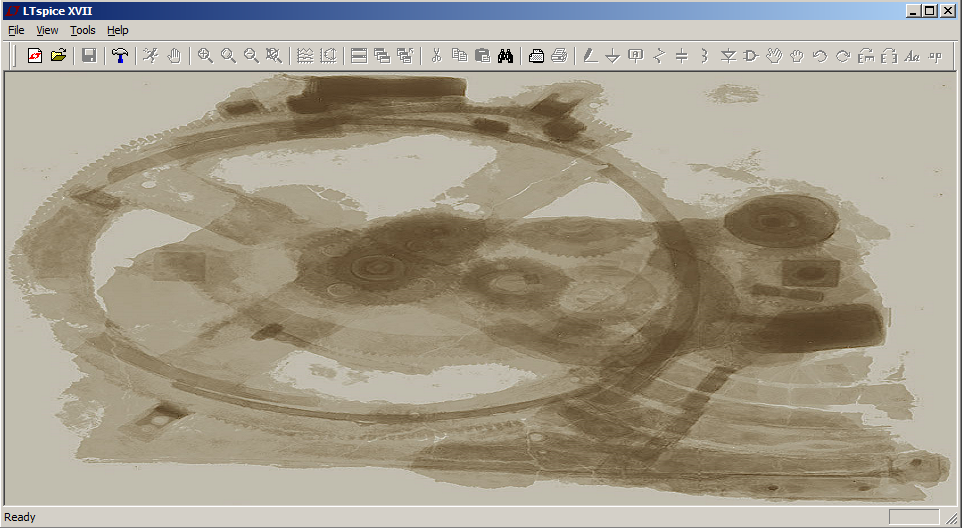
\includegraphics[width=\figwidth\textwidth]{figs/empty.png}
\caption{Графичко окружење}
\label{Fig:empty}
\end{figure}

Први корак, у сваком случају, јесте креирање нове шеме, тј. новог, празног, дијаграма, који ће се користити за цртање шеме. Кликом на иконицу \textit{New Schematic} (прва слијева у реду испод главног менија), добија се празна шема, као на слици~\ref{Fig:new}.

\begin{figure}[h]
\centering
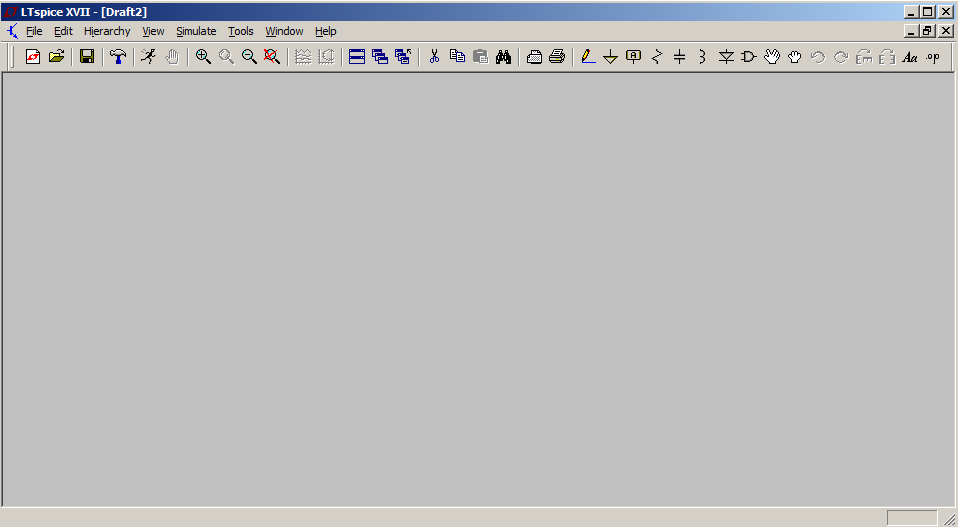
\includegraphics[width=\figwidth\textwidth]{figs/new.png}
\caption{Нова празна шема}
\label{Fig:new}
\end{figure}

За разлику од слике~\ref{Fig:empty}, на слици~\ref{Fig:new} јасно се види да су омогућене и друге иконице у реду испод главног менија. Оне представљају алате софтвера, како у вези са манипулацијом прозором и датотеком, тако и електричном шемом која се црта.

Предност \textit{LTSpice} је постојање пречица на тастатури за огромну већину акција, посебно оних најчешћих. Пречице су дате у форми табеле (\href{http://cds.linear.com/docs/en/software-and-simulation/LTspice_ShortcutFlyerC.pdf}{преузете одавдје\footnote{\url{http://cds.linear.com/docs/en/software-and-simulation/LTspice_ShortcutFlyerC.pdf}}}) на полеђини овог документа.

Нема потребе да се пречице на почетку уче напамет, довољно је да страна са пречицама буде доступна кориснику током рада - наравно, под условом, да се корисник заиста користи пречицама - па ће их упамтити рефлексивно. При том пречице су интуитивне - на примјер, ако је потребно додати отпорник у шему, довољно је притусни \textit{R}, а затим кликнути лијевим тастером миша на позицију гдје се елемент додаје. Тако је пречица за калем - \textit{L}, а за кондензатор - \textit{C}.

На једноставном примјеру демонстрирано је цртање шеме најважније шаблона у електричним склоповима - раздјелника напона. Прије почетка цртања, важно је имати у виду да се команда ,,један корак уназад'' (енгл. \textit{Undo}) задаје притиском на тастер \texttt{F9}.

\section{Цртање шеме раздјелника напона}
\label{rn}

Нека је прозор \textit{LTSpice} активан. Притиснте \textit{R} на тастури, а затим кликните лијевим тастером миша било гдје. Резултат ове двије операције приказан је на слици~\ref{Fig:rn-r1}.

\begin{figure}[h]
\centering
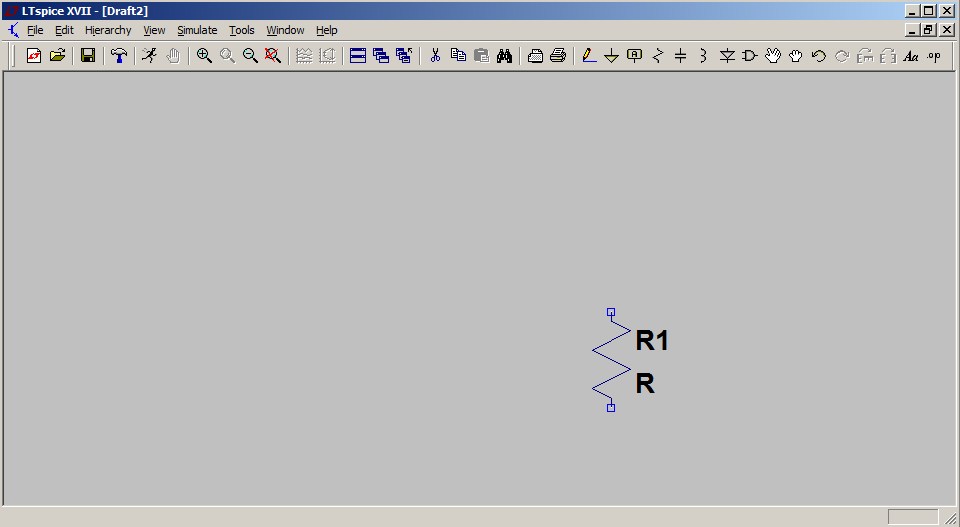
\includegraphics[width=\figwidth\textwidth]{figs/rn-r1.PNG}
\caption{Раздјелник напона - први отпорник}
\label{Fig:rn-r1}
\end{figure}

На тастатури притиснути тастере \texttt{Ctrl+R}, како би наредни отпорник био ротиран за $\nicefrac{\pi}{2}$. Потом још један клик лијевог миша за позиционирање, као на слици~\ref{Fig:rn-r2}.

\begin{figure}[h]
\centering
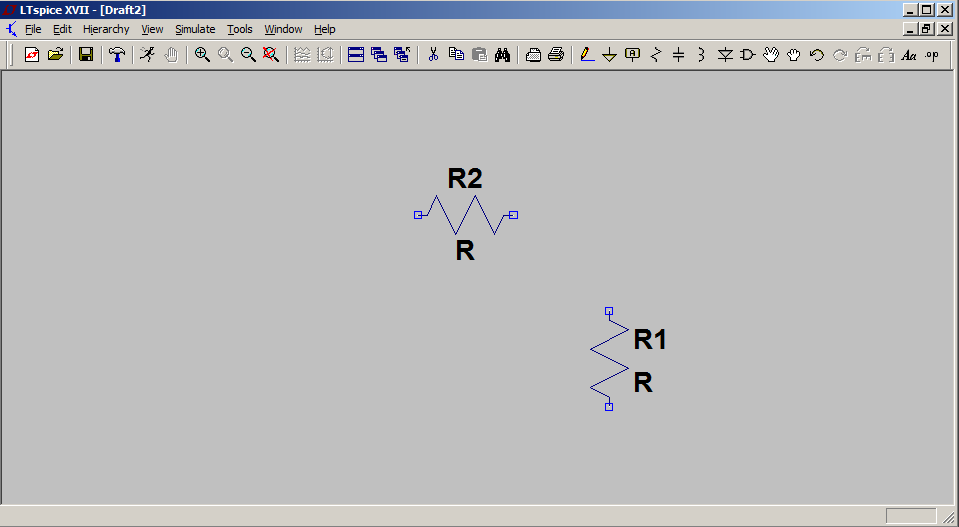
\includegraphics[width=\figwidth\textwidth]{figs/rn-r2.PNG}
\caption{Раздјелник напона - други отпорник}
\label{Fig:rn-r2}
\end{figure}

Посљедњи елемент потребан за напонски раздјелник је напонски извор. Пречица за ,,\textit{Нову компоненту}'' у општем случају јесте \texttt{F2}, па се може искористити у овом тренутку. Ова акција отвара прозор као на слици~\ref{Fig:rn-f2}.

\begin{figure}[h]
\centering
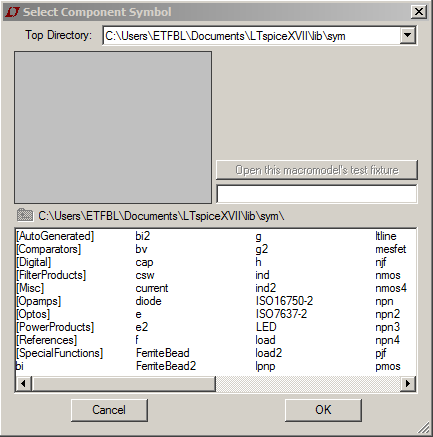
\includegraphics[width=0.5\textwidth]{figs/rn-f2.PNG}
\caption{Раздјелник напона - нова компонента у општем случају}
\label{Fig:rn-f2}
\end{figure}

Да би се изабрао напонски извор потребно је, одмах након \texttt{F2} на тастатури притиснути и тастере \texttt{vo} па \texttt{Enter}, и на крају још лијевим тастером миша позиционирати напонски извор на шему. Резултат ових акција приказан је на слици~\ref{Fig:rn-v}

\begin{figure}[h]
\centering
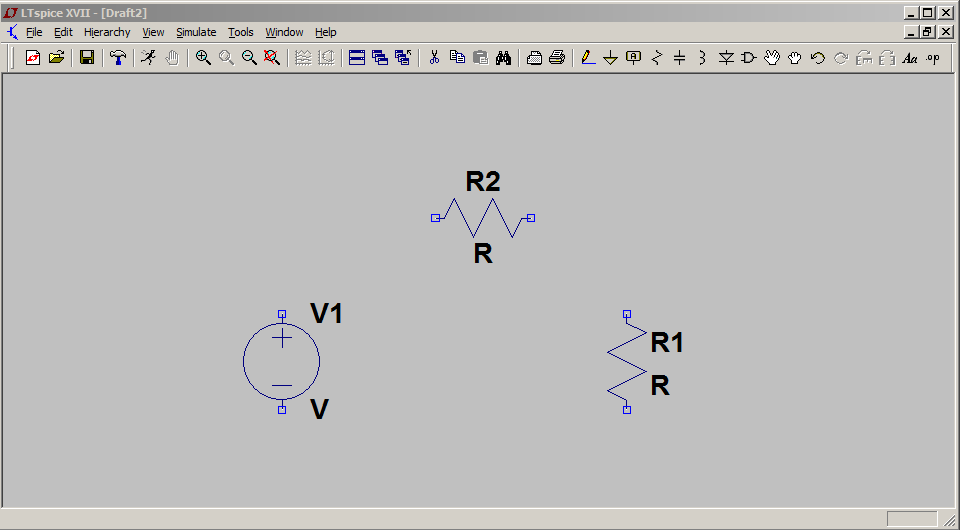
\includegraphics[width=\figwidth\textwidth]{figs/rn-v.PNG}
\caption{Раздјелник напона - напонски извор}
\label{Fig:rn-v}
\end{figure}

Сљедећи корак је успостављање веза између елемената, тј. дефинисање чворова електричне шеме. За почетак цртања линија везе, притиснути тастер \texttt{F3}, а затим кликнути на један од извода једног од елемената. На примјер, нека то буде горњи извод напонског извора. Са још два клика, спојити горњи извод напонског извора са лијевим изводом отпорника $R_2$. Иако ,,са још два клика'' звучи загонетно, чим се угледа изглед курсора (након притиска \texttt{F3}) и види његово понашање након првог клика (на горњи извод напонског извора), постаће јасно гдје треба да буду та два клика.

\begin{figure}[h]
\centering
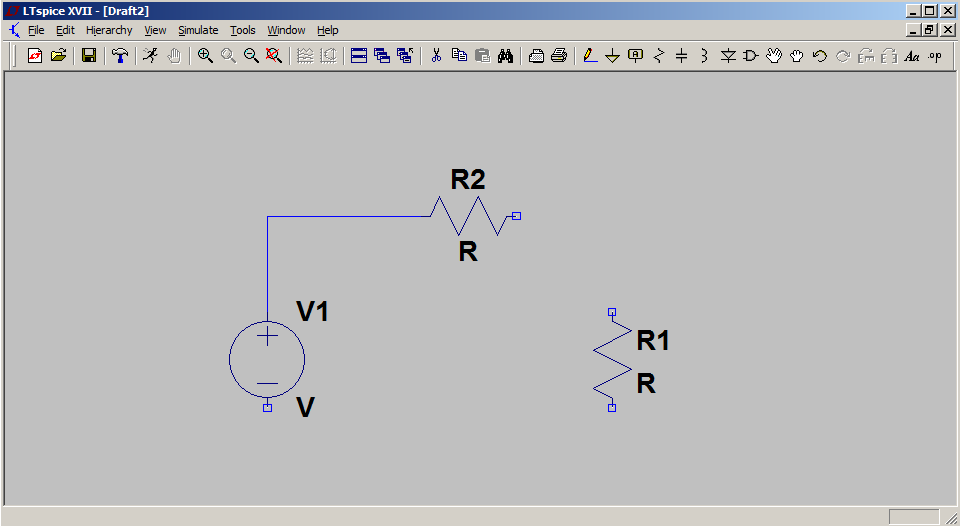
\includegraphics[width=\figwidth\textwidth]{figs/rn-n1.PNG}
\caption{Раздјелник напона - први чвор}
\label{Fig:rn-n1}
\end{figure}

Остале чворове у колу спојити, тако да коначан резултат буде као на слици~\ref{Fig:rn-n2}.

\begin{figure}[h]
\centering
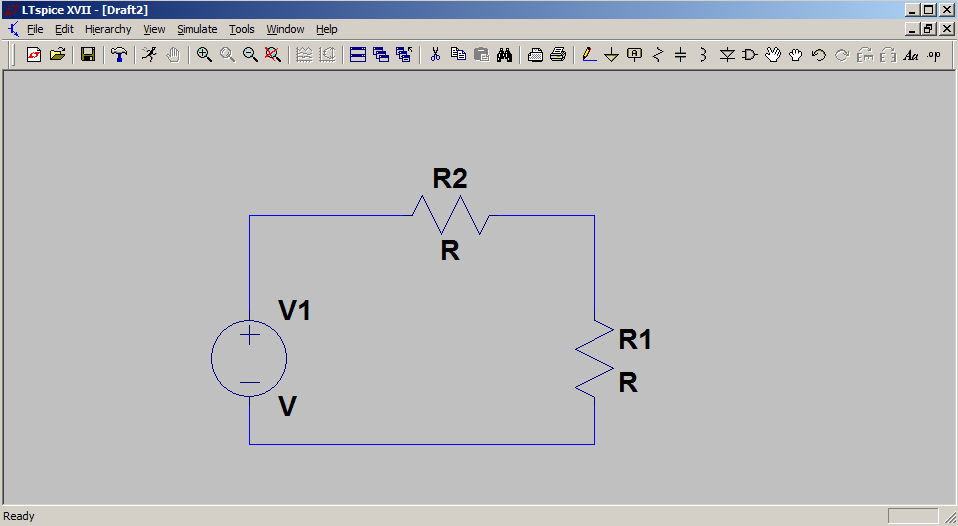
\includegraphics[width=\figwidth\textwidth]{figs/rn-n2.PNG}
\caption{Раздјелник напона - други чвор}
\label{Fig:rn-n2}
\end{figure}

Прије симулације, неопходно је и дефинисати нулти чвор, односно масу или уземљење, ткз. $GND$. Притиснути тастер \texttt{G} на тастатуре, а затим кликнути на одговарајући позицију. Резултат ове двије операције приказан је на слици~\ref{Fig:rn-g}. Наравно, шема није завршена, јер је неопходно спојити симбол нуле са једним од чворова кола. Нека то, на примјер, буде негативан извод напонског извора - метод је већ познат, користити тастер \texttt{F3}.

\begin{figure}[h]
\centering
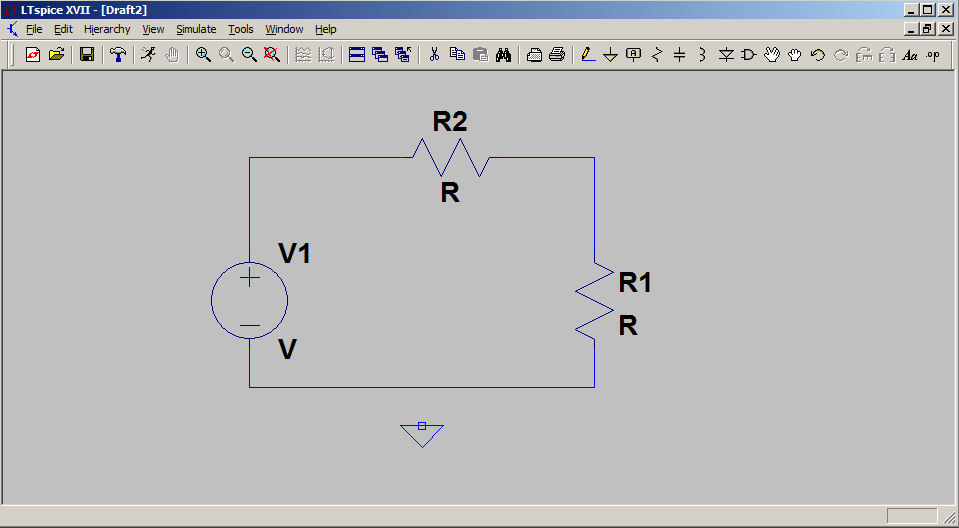
\includegraphics[width=\figwidth\textwidth]{figs/rn-g.PNG}
\caption{Раздјелник напона - нула, маса, уземљење, \textit{GND}}
\label{Fig:rn-g}
\end{figure}

Вриједности компонената уносе се на сљедећи начин. Десним тастером миша кликнути на отпорник $R_1$. Појављује се прозор као на слици~\ref{Fig:rn-rv1}, у којем је одмах активно поље \textit{Resistance}, па је довољно само наставити куцати потребну вриједност отпорника - нека то буде \texttt{10k}, а затим притиснути \texttt{Enter}.

\begin{figure}[h]
\centering
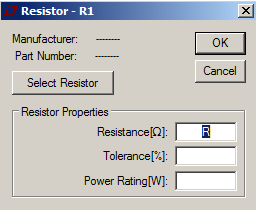
\includegraphics[width=0.4\textwidth]{figs/rn-rv1.PNG}
\caption{Раздјелник напона - прозор за унос вриједности отпорника}
\label{Fig:rn-rv1}
\end{figure}

Ове три акције поновити и над отпорником $R_2$ (с тим да је сада вриједност \texttt{20k}), што доводи до стања приказаног на слици~\ref{Fig:rn-rv2}.

\begin{figure}[h]
\centering
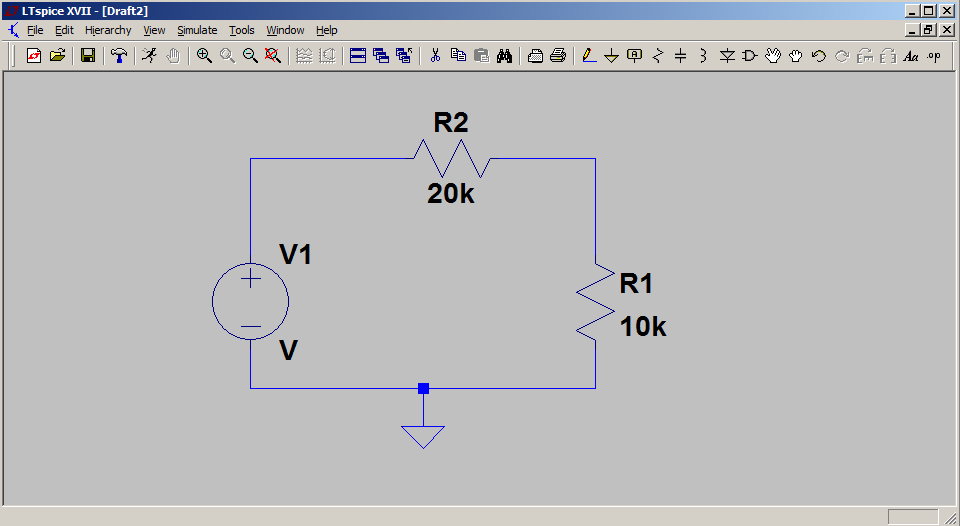
\includegraphics[width=\figwidth\textwidth]{figs/rn-rv2.PNG}
\caption{Раздјелник напона - унесене вриједности отпорника}
\label{Fig:rn-rv2}
\end{figure}

За унос вриједности напонског извора, искористити клик десног миша као и у претходна два случаја. На тај начин добија се прозор приказан на слици~\ref{Fig:rn-vv1}.

\begin{figure}[h]
\centering
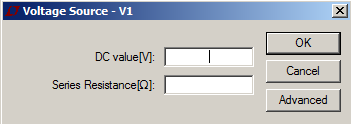
\includegraphics[width=0.5\textwidth]{figs/rn-vv1.PNG}
\caption{Раздјелник напона - прозор за унос вриједности напонског извора}
\label{Fig:rn-vv1}
\end{figure}

Унијети вриједност \texttt{12}, па притиснути \texttt{Enter}.

\begin{figure}[h]
\centering
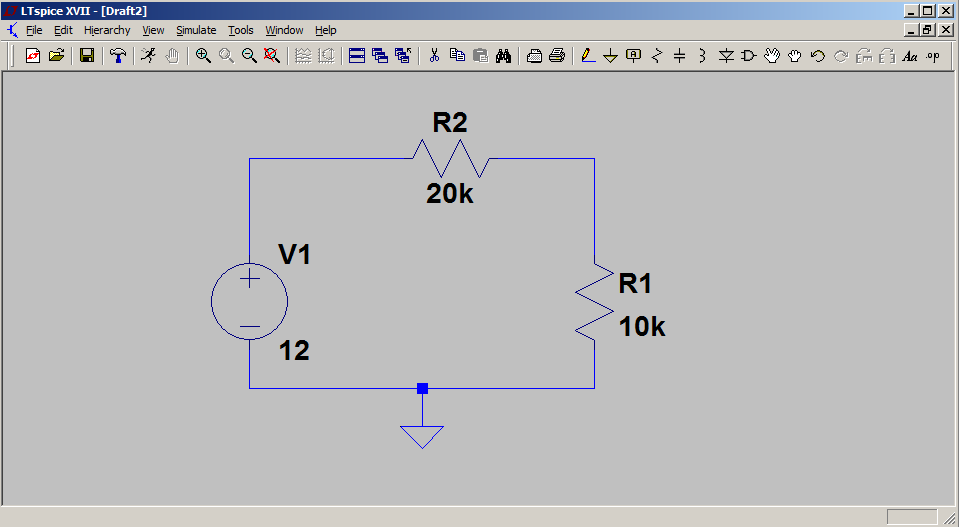
\includegraphics[width=\figwidth\textwidth]{figs/rn-vv2.PNG}
\caption{Раздјелник напона - унесене вриједности свих елемената}
\label{Fig:rn-vv2}
\end{figure}

Коначно, сви елементи су нацртани, сви чворови су спојени, назначен је нулти чвор, задате су вриједности свих елемената. Симулација може да почне.

\chapter{Симулације}
\label{sim}

У ревизији 2 \textit{Приручника} обрађени су сљедећи типови симулација:
\begin{enumerate}
\item симулација радне тачке,
\item симулација понашања кола при промјени напона једносмјерног напона,
\item временска анализа, одзив на импулсну побуду.
\end{enumerate}

\section{Симулација радне тачке}
\label{op}

Настављајући рад на пројекту раздјелника напона привремено заустављен при стању приказаном на слици~\ref{Fig:rn-vv2}, треба да се подесе параметри симулатора. Кликом на иконицу пету слијева испод главног менија, \textit{Run}, добија се прозор као на слици~\ref{Fig:rn-tran0}, са више језичака.

\begin{figure}[h]
\centering
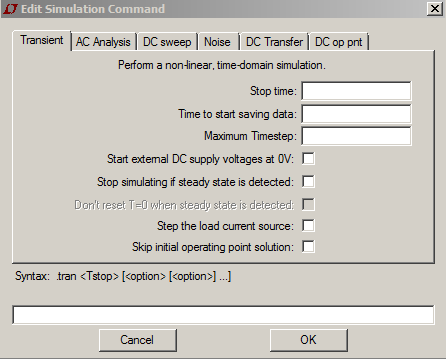
\includegraphics[width=0.5\textwidth]{figs/rn-tran0.PNG}
\caption{Подешавање временске симулације - подразумијевано активни језичак прозора за подешавање симулације}
\label{Fig:rn-tran0}
\end{figure}

Тренутно активни језичак посвећен је подешавању временске (транзијентне) симулације, па није од интереса у оквиру овог пододјељка. Симулација радне тачке подешава се посљедњим језичком у низу, насловљеним \textit{DC op pnt}. Кликом изабрати тај језичак, чиме се добија прозор као на слици~\ref{Fig:rn-op0}.

\begin{figure}[h]
\centering
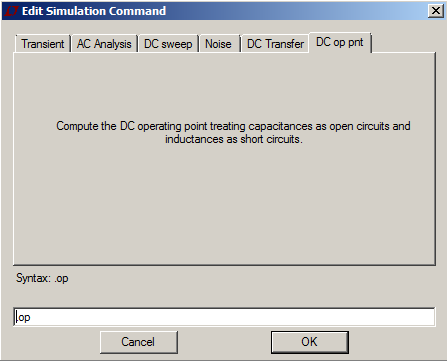
\includegraphics[width=0.5\textwidth]{figs/rn-op0.PNG}
\caption{Раздјелник напона - подешавање симулације радне тачке}
\label{Fig:rn-op0}
\end{figure}

Очигледно, овдје нема потребе ни за каквим подешавањима. То има смисла и у контексту чињенице да је ово симулација намијењена искључиво једносмјерној анализи при тачно одређеним вриједностима компонената, и то при тачно једној вриједности за сваки од параметара. Зато је сљедећа акција лијевим тастером миша кликнути \texttt{OK}. 

Одмах потом добија се текстуални испис рјешења у форми као на слици~\ref{Fig:rn-op1}.

\begin{figure}[h]
\centering
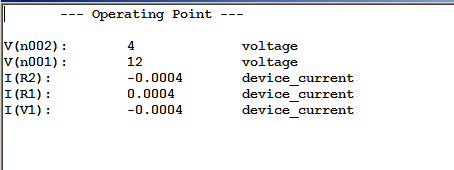
\includegraphics[width=0.5\textwidth]{figs/rn-op1.PNG}
\caption{Раздјелник напона - текстуални испис резултата симулације радне тачке}
\label{Fig:rn-op1}
\end{figure}

Након клика \texttt{OK} и шема је измијењена, па се, након затварања текстуалног исписа рјешења, у прозору за цртање шеме види стање као на слици~\ref{Fig:rn-op2}. Наиме, појављује се \textit{Spice} директива \texttt{.op}, што је у ствари текстуални начин издавања наредбе симулатору да уради симулацију радне тачке.

\begin{figure}[h]
\centering
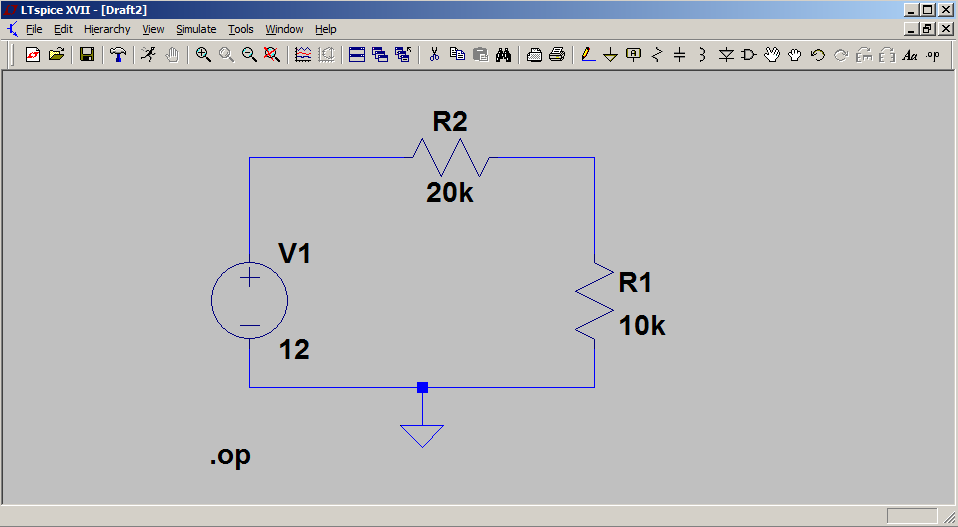
\includegraphics[width=\figwidth\textwidth]{figs/rn-op2.PNG}
\caption{Раздјелник напона - \textit{Spice} директива за симулацију радне тачке}
\label{Fig:rn-op2}
\end{figure}

Шема је постала интерактивна, што је могуће потврдити постављањем показивача миша (још увијек не кликнути) на неки од чворова или елемената. Ако се, на примјер, постави показивач миша на чвор између два отпорника у доњој траци прозора софтвера (енгл. \textit{Status Bar}) видјеће се износ напона. Такође, показивањем на отпорник, у доњој траци прозора се виде информације у вези са струјом кроз њега, те његовом снагом дисипације.

Кликом на чвор између два отпорника (показивач миша умјесто крстића поприма облик црвене сонде) на шеми се исписује вриједност једносмјерног напона тог чвора - добијена као резултат симулације. Наравно, то се може урадити и за преостале чворове у колу, па се добија ситуација као на слици~\ref{Fig:rn-op3}.

\begin{figure}[h]
\centering
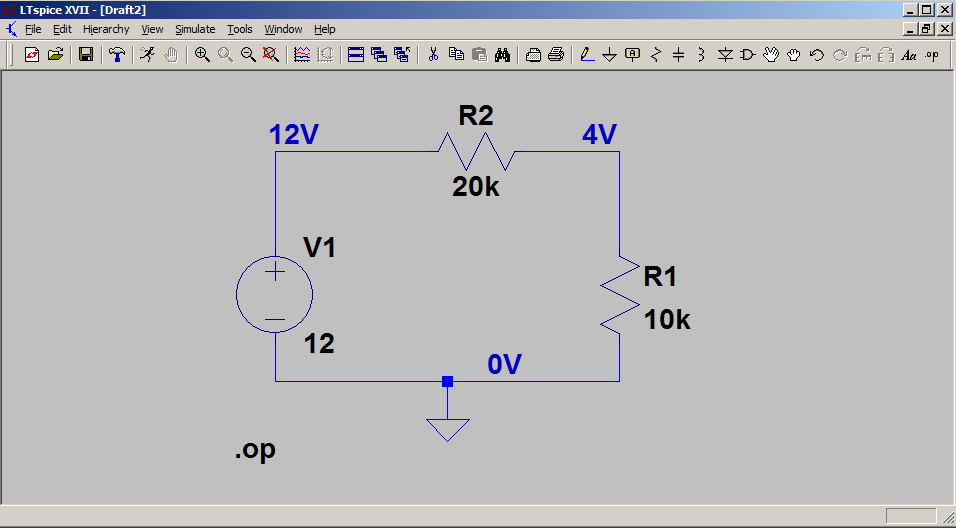
\includegraphics[width=\figwidth\textwidth]{figs/rn-op3.PNG}
\caption{Раздјелник напона - приказивање резултата симулације радне тачке на шеми}
\label{Fig:rn-op3}
\end{figure}

\section{Симулација промјене једносмјерног напона}
\label{dc}

Задржавши пројекат симулиран у одјељку~\ref{op} отвореним, врста симулације се може измијенити на два начина:
\begin{enumerate}
\item избором: \textit{Simulate $\rightarrow$ Edit Simulation Cmd}, односно
\item десним кликом на постојећу команду \texttt{.op}.
\end{enumerate}
Оба ова потеза отварају прозор приказан на слици~\ref{Fig:rn-op0}. Избором језичка \texttt{DC sweep}, добија се прозор као на слици~\ref{Fig:rn-dc0}

\begin{figure}[h]
\centering
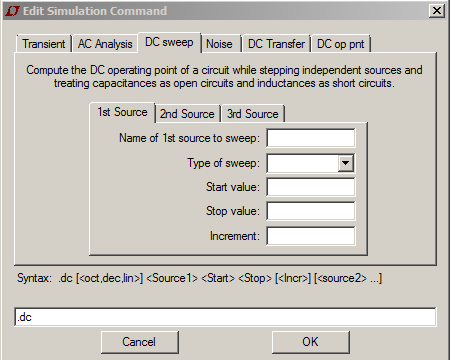
\includegraphics[width=0.5\textwidth]{figs/rn-dc0.PNG}
\caption{Раздјелник напона - подешавање симулације промјене једносмјерног напона}
\label{Fig:rn-dc0}
\end{figure}

На овај начин могуће је независно мијењати до три напонска извора, а у наставку је дат примјер промјене једног, будући да је за остале приступ аналоган. Прво је потрено унијети назив извора чији напон ће се мијењати. У случају раздјелника напона, то је \texttt{V1}. 

Затим се бира врста корака симулације: линеаран, по октави или декади, те конкретне вриједности у форми листе. Свака од ове четири могућности има своју примјену, која често зависи од врсте кола и врсте симулације. У случају једномјерних напона, најчешће је интересантно посматрати линеарну промјену, па је то избор и у овом случају.

Наредна два поља служе за уност почетне и крајње вриједности напона, тј. граничних вриједности напона у оквиру којих ће се напон генератора \texttt{V1} мијењати. Разлика крајње и почетне вриједности назива се опсег. Посљедње поље представља корак симулатора, тј. размак између двије тачке у којима софтвер прорачунава напоне и струје кола. Да би резултати симулације били смислени, неопходно је да ова вриједност буде пригодно изабрана, а то значи много мања од опсега - конкретно, треба да буде најмање десет пута мања од опсега, а често и до 100 или више пута мања. Наравно, ово је само почетна вриједност за корак, те није искључено да се у наредној итерацији симулације кола вриједност корака прилагођава. Нека су почетна и крајња вриједност \texttt{0 V} и \texttt{5 V}, а корак, у складу са претходном дискусијом, \texttt{0.5 V}

Примјетно је како се, током попуњавања ових поља, у пољу на дну прозора аутоматски попуњава \textit{Spice} директива за ову врсту симулације. По завршеном уносу, прозор изгледа као на слици~\ref{Fig:rn-dc1}. Избором тастера \texttt{OK}, шема је модификована новом директивом и коначан изглед приказан је на слици~\ref{Fig:rn-dc2}.

\begin{figure}[h]
\centering
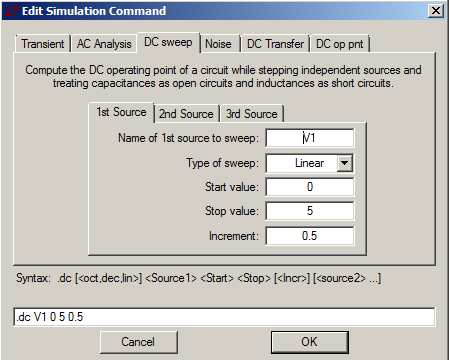
\includegraphics[width=0.5\textwidth]{figs/rn-dc1.PNG}
\caption{Раздјелник напона - подешавање симулације промјене једносмјерног напона, унесене вриједности}
\label{Fig:rn-dc1}
\end{figure}

\begin{figure}[h]
\centering
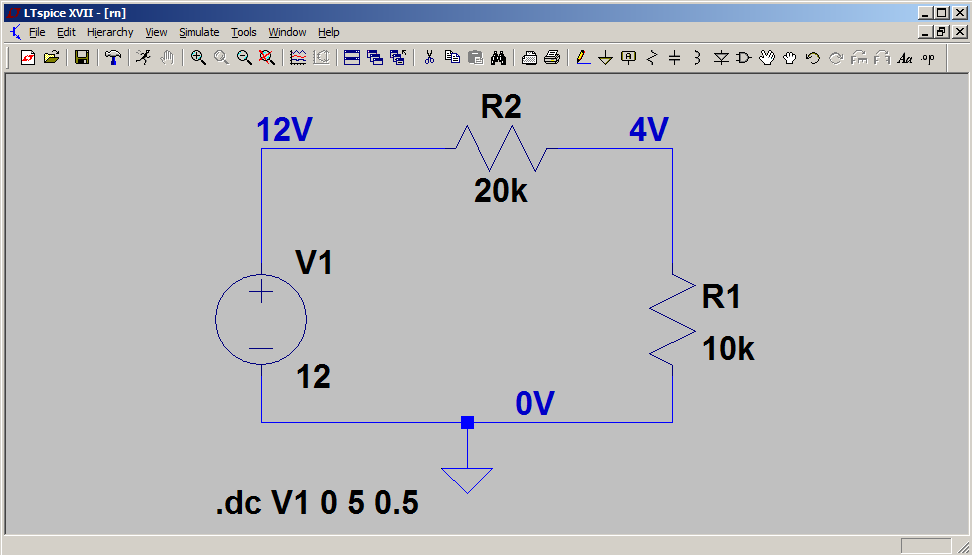
\includegraphics[width=\figwidth\textwidth]{figs/rn-dc2.PNG}
\caption{Раздјелник напона - \textit{Spice} директива за симулацију промејене једносмјерног напона}
\label{Fig:rn-dc2}
\end{figure}

Симулација се покреће на познат начин, а након успјешног завршетка, прозор симулатора подијељен је на два хоризонтална дијела, као на слици~\ref{Fig:rn-dc3}. Горњи прозор црне позадине служи за графички приказ резултата симулације. Апсциса представља промјену улазне величине - што је у овом случају напон генератора \texttt{V1}. Ордината у почетку није дефинисана, па тренутно и нема ознаке. Да би и ордината добила значење, потребно је изабрати величину са шеме (напон или струју) која ће се посматрати. Лијевим кликом на позитиван крај генератора напона \texttt{V1}, у прозору за графички приказ добија се промјена напона тог чвора у зависности од промјене напона генератора. Наравно, с обзиром да се ради о истом напону, добија се крива нагиба 1, као на слици~\ref{Fig:rn-dc4}

\begin{figure}[h]
\centering
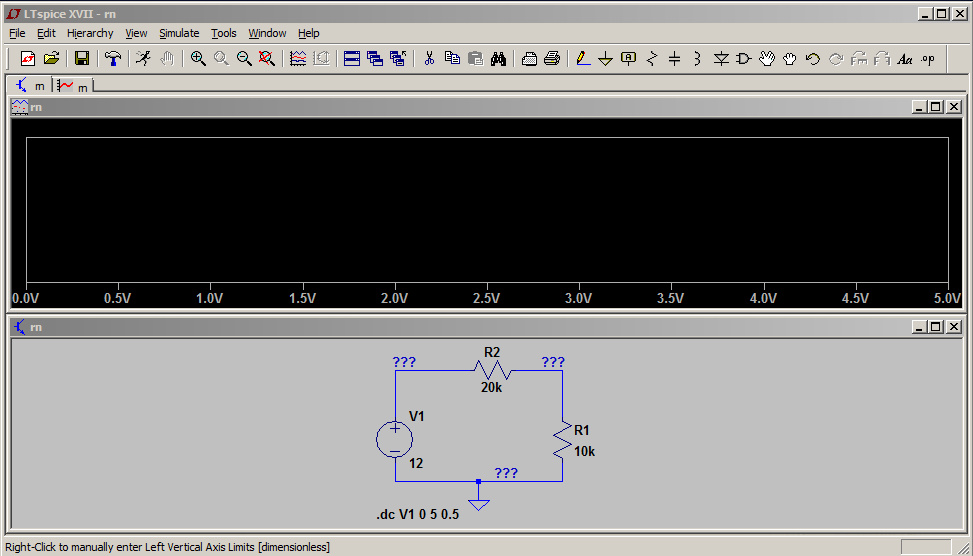
\includegraphics[width=\figwidth\textwidth]{figs/rn-dc3.PNG}
\caption{Раздјелник напона - завршена симулација}
\label{Fig:rn-dc3}
\end{figure}

\begin{figure}[h]
\centering
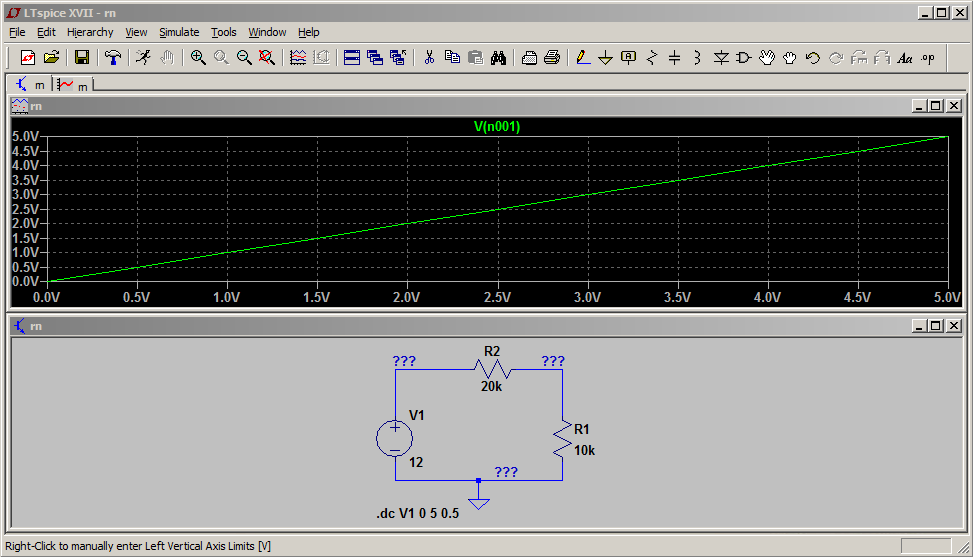
\includegraphics[width=\figwidth\textwidth]{figs/rn-dc4.PNG}
\caption{Раздјелник напона - приказ промјене напона генератора, тј. напона на улазу раздјелника}
\label{Fig:rn-dc4}
\end{figure}

Да би се добила информација о излазном напону, потребно је лијевим тастером миша кликнути на чвор између два отпорника - тај напон се може сматрати излазним напоном када је у питању раздјелник напона. Одмах се у горњем прозору појављује и плава линија која осликава зависност излаза раздјелника напона од промјене улазног напона, као на слици~\ref{Fig:rn-dc5}.

\begin{figure}[h]
\centering
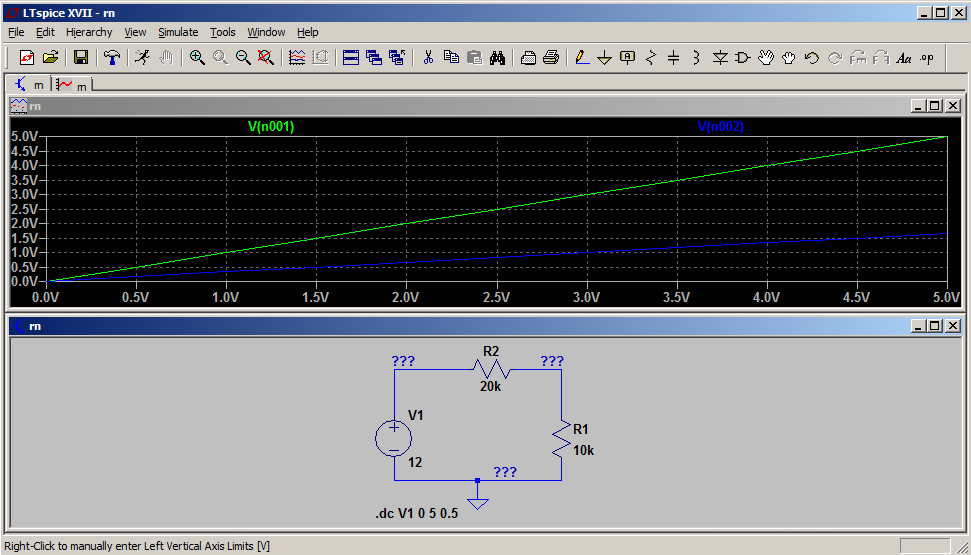
\includegraphics[width=\figwidth\textwidth]{figs/rn-dc5.PNG}
\caption{Раздјелник напона - приказ промјене напона на излазу раздјелника}
\label{Fig:rn-dc5}
\end{figure}

\section{Временска анализа}
\label{tran}

Да би се анализирало понашање електричног кола у зависности од протока времена, неопходно је промијенити промјенљиву симулације. У претходном случају промјенљива симулације био је напон генератора. Другим ријечима, коло је рјешавано за сваки од корака дефинисаних приликом подешавања симулације, али увијек у истом временском тренутку, тј. у еквилибријуму и независно од протока времена. У овом одјељку, главна промјенљива симулације је вријеме.

Временску анализу могуће је извршити користећи једносмјерне напонске изворе (какав је био \texttt{V1} кориштен у одјељку~\ref{dc}). Ипак, такви извори се користе искључиво као напајања или референце, док је за побуду неопходно користити извор који је такође функција времена. Тек је на тај начин могуће посматрати одзив кола у времену - било на простопериодичну или импулсну побуду.

За потребе демонстрације временске анализе кориштењем симулатора \textit{LTspice} припремљено је \textit{RC} коло као на слици\ref{Fig:rc-t0}. Знајући да су и отпорник и кондензатор, у ствари, двије врсте импедансе, и ово коло се може посматрати као раздјелник напона.

\begin{figure}[h]
\centering
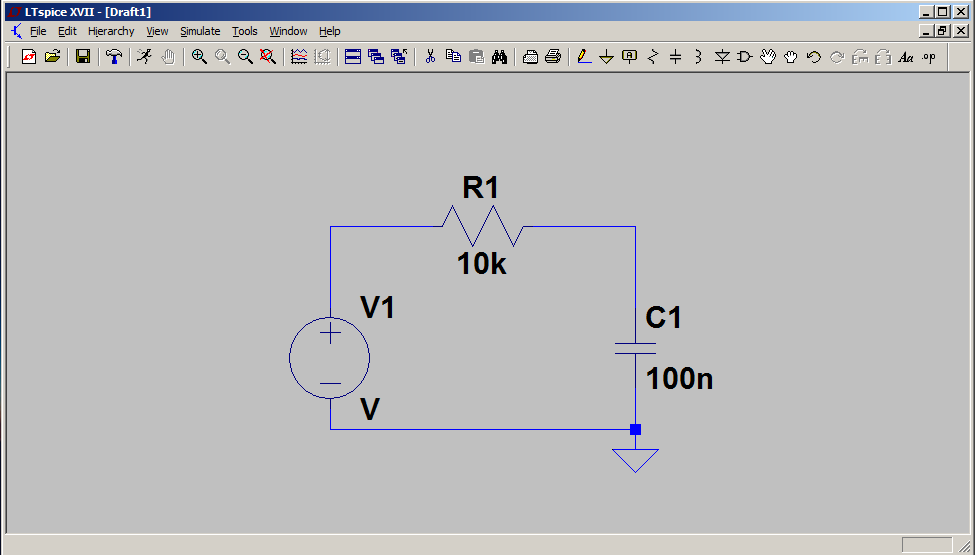
\includegraphics[width=\figwidth\textwidth]{figs/rc-t0.PNG}
\caption{Раздјелник напона - \textit{RC} коло}
\label{Fig:rc-t0}
\end{figure}

На претходној слици унесене су вриједност оба пасивна елемента, али је генератор напона остао недефинисан - зато што је потребно унијети параметре импулсне побуде. Десним кликом на генератор добија се прозор као на слици~\ref{Fig:rn-v}. У овом прозору могуће је подесити само генератор једносмјерног напона, па је за остале врсте генератора потребно клкнути на тастер \texttt{Advanced}. Прозор који се добија приказан је на слици~\ref{Fig:rc-t1}

\begin{figure}[h]
\centering
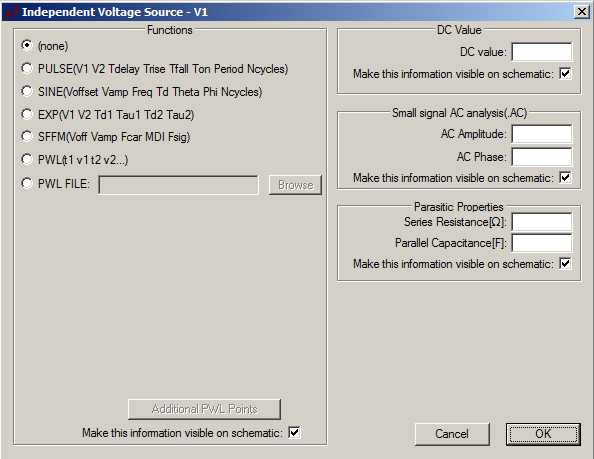
\includegraphics[width=0.7\textwidth]{figs/rc-t1.PNG}
\caption{Подешавање напредних опција генератора}
\label{Fig:rc-t1}
\end{figure}

За подешавање генератора импулсне побуде бира се друга по реду опција, као на слици~\ref{Fig:rc-t2}.

\begin{figure}[h]
\centering
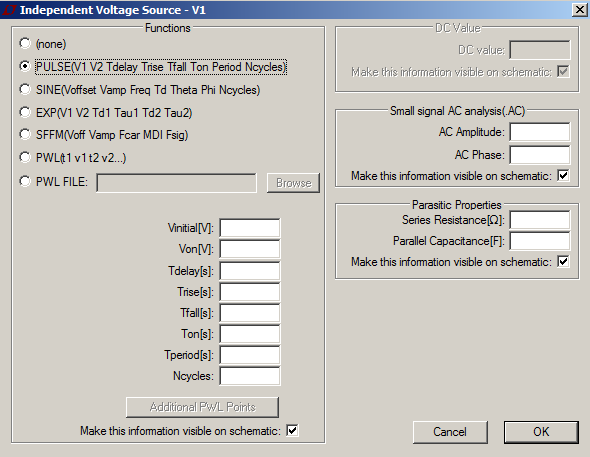
\includegraphics[width=0.7\textwidth]{figs/rc-t2.PNG}
\caption{Подешавање генератора импулсне побуде}
\label{Fig:rc-t2}
\end{figure}

Да би се добила импулсна побуда параметри које је неопходно унијети су:
\begin{enumerate}
\item напонски ниво прије почетка импулса, тј. почетни напон,
\item напонски ниво током трајања импулса, тј. напон када је генератор укључен,
\item вријеме задржавања, тј. вријеме до почетка импулса,
\item вријеме раста, тј. вријеме од почетка раста напона генератора од почетног напона до напонског нивоа током трајања импулса,
\item вријеме пада, тј. вријеме од почетка опадања напонског нивоа импулса, до почетног напона,
\item вријеме трајања импулса, тј. вријеме трајања укљученог стања генератора,
\item период понављања.
\end{enumerate}

Нека су унесене вриједности као на слици~\ref{Fig:rc-t3}, те потврђене кликом \texttt{OK}.

\begin{figure}[h]
\centering
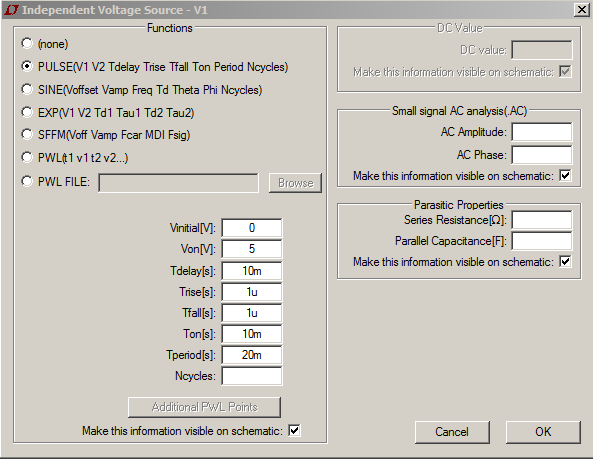
\includegraphics[width=0.7\textwidth]{figs/rc-t3.PNG}
\caption{Подешавање генератора импулсне побуде - унесене вриједности}
\label{Fig:rc-t3}
\end{figure}

Сљедећи корак је подашавање временске анализе. Почетни прозор подешавања симулације приказан је на слици~\ref{Fig:rn-tran0}, и подразумијевано отвара језичак за подешавање временске анализе. Најважнији параметар је вријеме до којег ће симулатор пратити понашање кола. Могуће је дефинисати и корак, те још неке напредне опције, али нека су, у овом случају, унесене вриједности као на слици~\ref{Fig:rc-t4}, те потврђене кликом \texttt{OK}.

\begin{figure}[h]
\centering
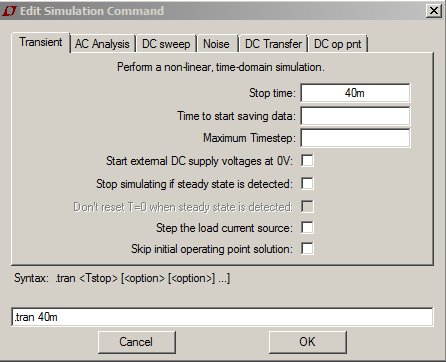
\includegraphics[width=0.7\textwidth]{figs/rc-t4.PNG}
\caption{Подешавање временске анализе - унесене вриједности}
\label{Fig:rc-t4}
\end{figure}

Коло је, сада, спремно за симулацију, али због лакшег сналажења међу таласним облцима који ће се јавити као резултати временске анализе, могуће је именовати чворове. Притиском на тастер \texttt{F4} тастатуре, добија се прозор као на слици~\ref{Fig:rc-t5}.

\begin{figure}[h]
\centering
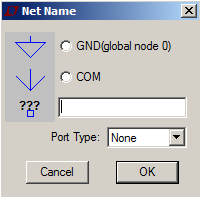
\includegraphics[width=0.3\textwidth]{figs/rc-t5.PNG}
\caption{Унос назива чвора}
\label{Fig:rc-t5}
\end{figure}

Нека се улазни чвор зове \texttt{vin} а излазни \texttt{vout}. Да би се то име додијелило чвору, унесе се у отворени прозор, кликне \texttt{OK}, а затим кликне на жељени чвор. Радњу поновити и за други чвор. Коначан изглед шеме дат је на слици~\ref{Fig:rc-t6}.

\begin{figure}[h]
\centering
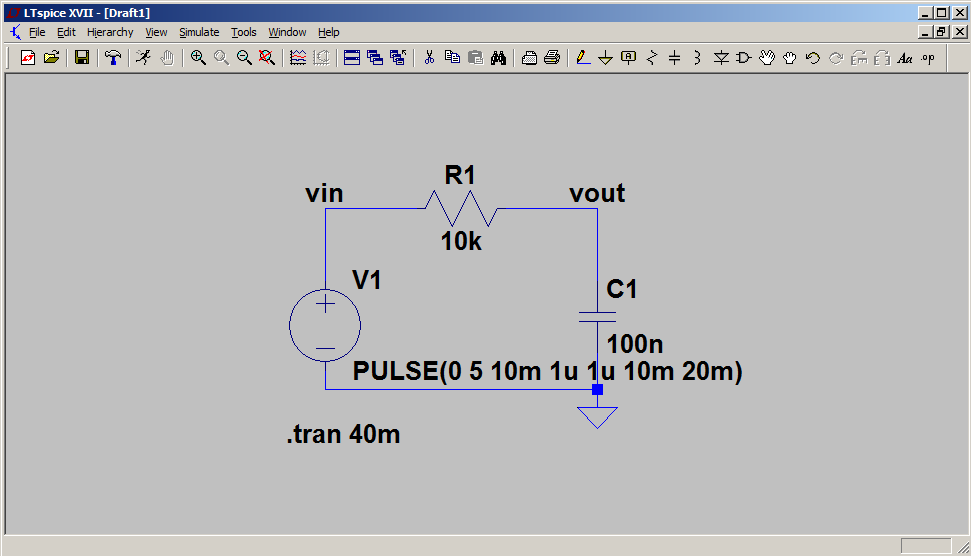
\includegraphics[width=\figwidth\textwidth]{figs/rc-t6.PNG}
\caption{Раздјелник напона - \textit{RC} коло - коначан изглед}
\label{Fig:rc-t6}
\end{figure}

Након успјешног покретања и завршетка симулације, добра пракса је увијек увјерити се да се напонски извор понаша како је предвиђено. Због тога је први корак приказ таласног облика напона на позитивном крају напонског извора. Резултат ове акције приказан је на слици~\ref{Fig:rc-t7}.

\begin{figure}[h]
\centering
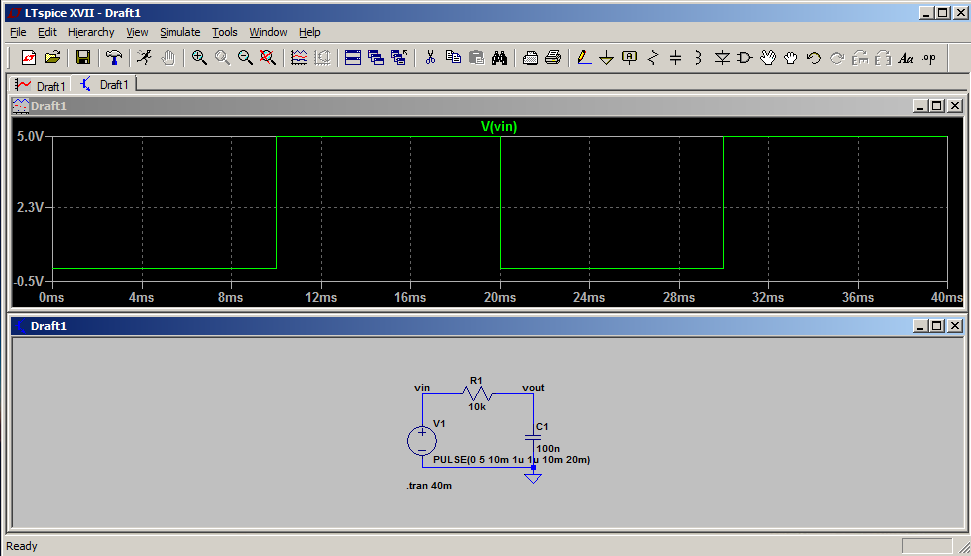
\includegraphics[width=\figwidth\textwidth]{figs/rc-t7.PNG}
\caption{Раздјелник напона - \textit{RC} коло - таласни облик улазног напона}
\label{Fig:rc-t7}
\end{figure}

Коначно, таласни облик излазног напона, рјешење кола у свим временским тренуцима од \texttt{t=0} до \texttt{t=40 ms}, добија се кликом на чвор \texttt{vout}, а приказан је на слици~\ref{Fig:rc-t8}.

\begin{figure}[h]
\centering
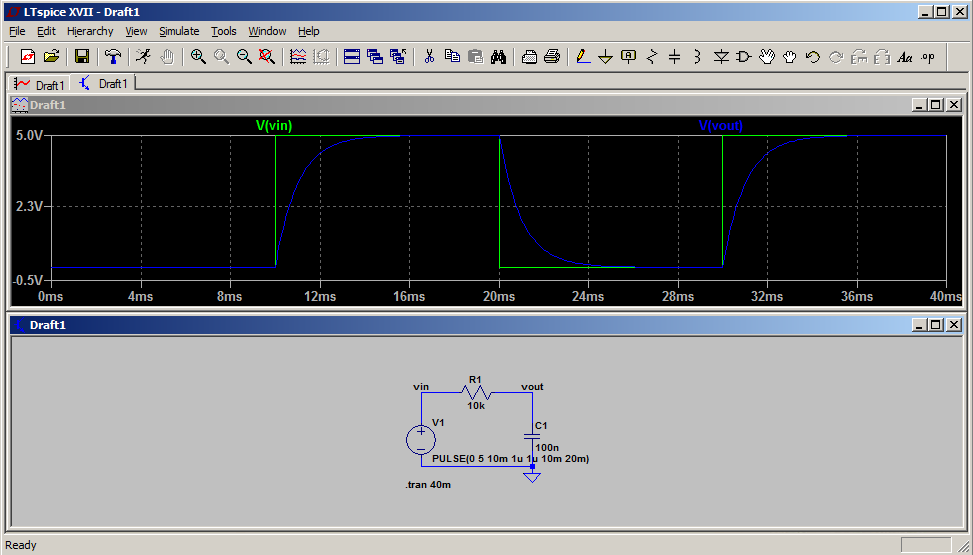
\includegraphics[width=\figwidth\textwidth]{figs/rc-t8.PNG}
\caption{Раздјелник напона - \textit{RC} коло - резултати симулације, талсни облик излазног напона}
\label{Fig:rc-t8}
\end{figure}

\section{Параметарска анализа}
\label{param}

Симулација електричног кола је један вид аутоматизације рјешњавања електричног кола. У досадашњим одјељцима аутоматизовани су два процеса: исписивање једначина кола, те рјешавање тих једначина - односно добијање струја и напона кола.

У одјељку~\ref{dc} показано је како исто коло ријешити у више итерација, при чему је у свакој итерацији мијењан напон улазног једносмјерног генератора. Тако је на слици~\ref{Fig:rn-dc5} приказано рјешење (,,излазни'' напон раздјелника напона) за сваку задату вриједност улазног генератора напона \texttt{V1}. Тако је уведена додатна димензија аутоматизације - тј. умјесто да се покреће 10 пута симулација радне тачке (одјељак~\ref{op}), покренута је једна симулација промјене једносмјерног напона, а резултат приказан графички. 

И временска анализа се може посматрати у истом контексту. Умјесто да се коло са слике~\ref{Fig:rc-t0} рјешава за сваки временски тренутак ручно водећи рачуна о тренутној вриједности напона улазног генератора, покренута је једна симулација која итеративно рјешава коло, водећи рачуна о вриједности напона улазног генератора у сваком временском тренутку.

У оба ова случаја, вриједност компонената је константна - отпорности и капацитивности су увијек исте. Понекад је интересантно посматрати како се одзив кола понаша у зависности од промјене вриједности компоненте. Могуће је, наравно, покренути три симулације у временском домену за коло са слике~\ref{Fig:rc-t0} прије сваког покретања мијењајући капацитивност тако да износи 100~nF, 1~\textmugreek F и 10~\textmugreek F. 

Овај поступак се аутоматизује кориштењем \textit{Spice} команде (директиве) \texttt{STEP}. Прилагодити шему и резултат приказан на~\ref{Fig:rc-t8} тако да одговара слици~\ref{Fig:rc-step0}.

\begin{figure}[h]
\centering
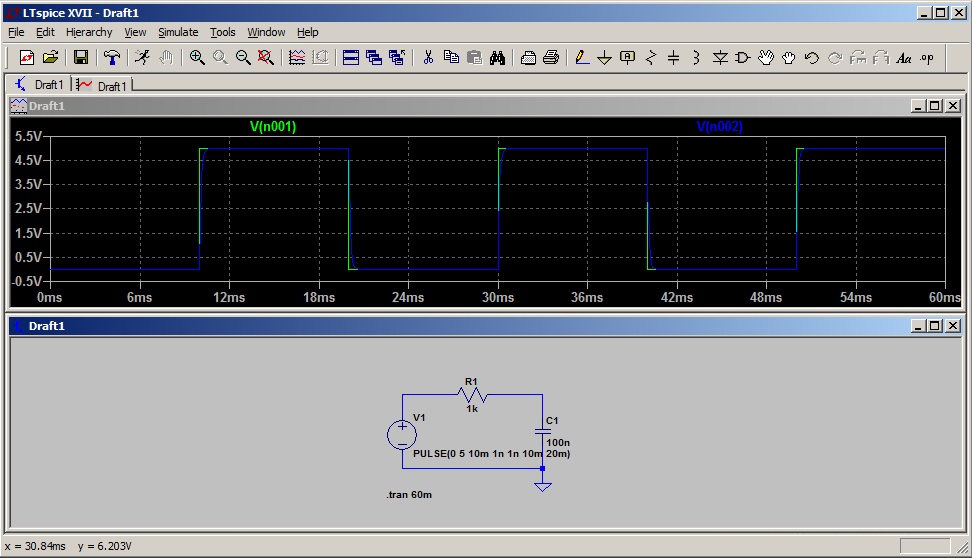
\includegraphics[width=\figwidth\textwidth]{figs/rc-step0.PNG}
\caption{Резултати симулације \textit{RC} кола}
\label{Fig:rc-step0}
\end{figure}

Да би вриједност компоненте била промјенљива, неопходно је дефинисати промјенљиву (варијаблу), односно параметар који се мијења у различитим итерацијама симулације. Десним тастером миша кликнути на компоненту чију је вриједност потребно мијењати итеративно. Параметар, односно промјенљива симулације се дефинише тако што се њен назив у витичастим заградама унесе умјесто вриједности капацитивности, као на слици~\ref{Fig:rc-step1}. Притиснути \texttt{Enter} или кликнути \texttt{OK}.

\begin{figure}[h]
\centering
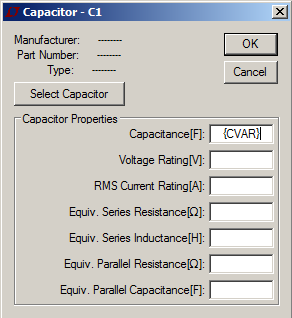
\includegraphics[width=0.3\textwidth]{figs/rc-step1.PNG}
\caption{Резултати симулације \textit{RC} кола}
\label{Fig:rc-step1}
\end{figure}

Сада је потребно дефинисати опсег управо креиране промјенљиве, те начин промјене унутар тог опсега. Притиском на тастер \texttt{S} тастатуре, добија се дијалог као на слици~\ref{Fig:rc-step2}. У ово поље уносе се \textit{Spice} директиве, одосно команде, па тако и поменута \texttt{STEP}. 

\begin{figure}[h]
\centering
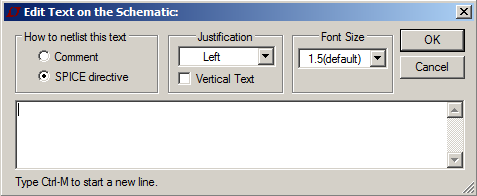
\includegraphics[width=0.5\textwidth]{figs/rc-step2.PNG}
\caption{Резултати симулације \textit{RC} кола}
\label{Fig:rc-step2}
\end{figure}

Нека су вриједности кондензатора од интереса три наведене прије неколико пасуса. У поље дијалога са претходне слике унијети:

\begin{center}
\texttt{.step param CVAR list 100n 1u 10u}
\end{center}

Ова директива би се могла превести псеудо-к\^{о}дом како слиједи:

\vspace{6pt}
\noindent\texttt{int CVAR[3] = \{100n, 1u, 10u\}}

\noindent\texttt{for(int i = 0; i < 3; i++)}

\hspace{48pt}\texttt{\{Run simulation at C1=CVAR[i]\}}
\vspace{6pt}

Другим ријечима, дакле: ,,за сваку од вриједности у низу \texttt{CVAR} покренути исту симулацију''.

Користећи се опцијама \texttt{Move} и \texttt{Drag} довести шему у стање као на слици~\ref{Fig:rc-step3}.

\begin{figure}[h]
\centering
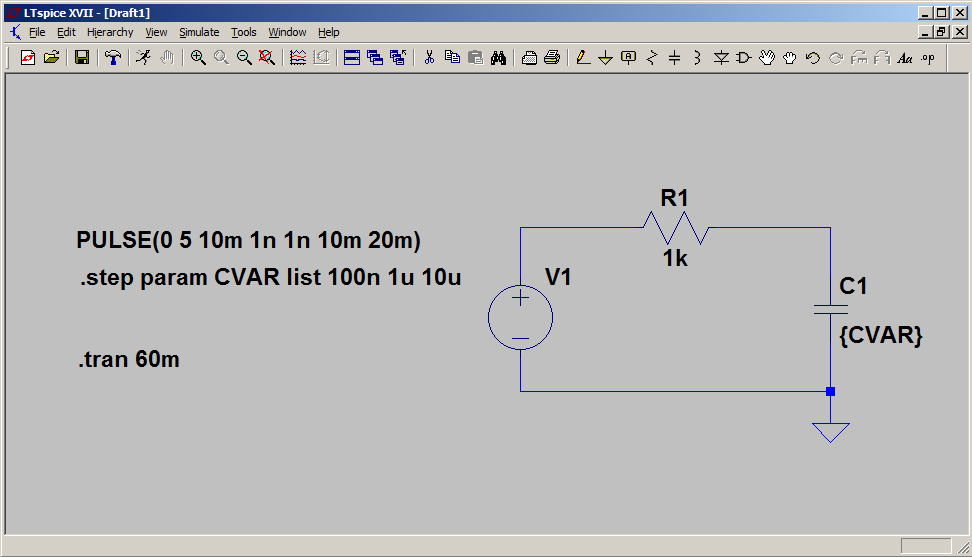
\includegraphics[width=\figwidth\textwidth]{figs/rc-step3.PNG}
\caption{Резултати симулације \textit{RC} кола}
\label{Fig:rc-step3}
\end{figure}

Покретање симулације даје резултате као на слици~\ref{Fig:rc-step4}.

\begin{figure}[h]
\centering
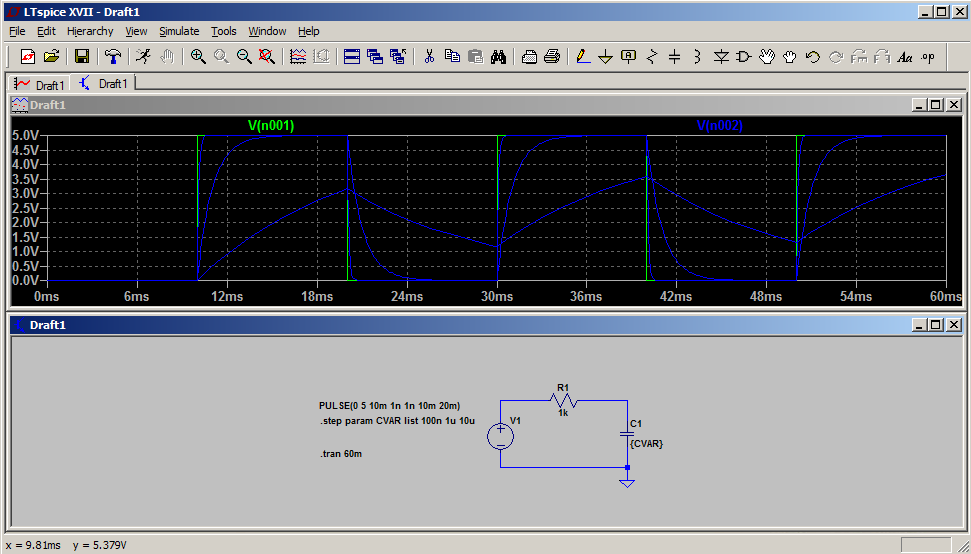
\includegraphics[width=\figwidth\textwidth]{figs/rc-step4.PNG}
\caption{Резултати симулације \textit{RC} кола}
\label{Fig:rc-step4}
\end{figure}

Други начин задавања промјене унутар опсега вриједности је приказан на слици~\ref{Fig:rc-step5} и аналоган је задављу промјене једносмјерног напона описаног у одјељку~\ref{dc}.

\begin{figure}[h]
\centering
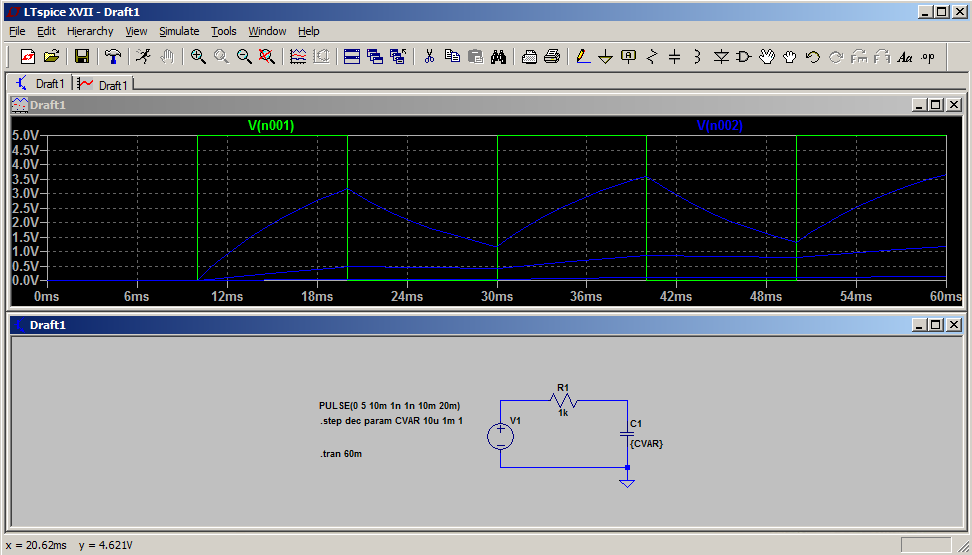
\includegraphics[width=\figwidth\textwidth]{figs/rc-step5.PNG}
\caption{Резултати симулације \textit{RC} кола}
\label{Fig:rc-step5}
\end{figure}

\section{Фреквенцијска анализа}

Фреквенцијска анализа је још један вид аутоматизације, с тим да се у овом случају симулације итеративно врше за различите учестаности. Прво је потребно улазни генератор са слике~\ref{Fig:rc-t8} прилагодити - довести га у стање као што је приказано на слици~\ref{Fig:rc-ac0}.

\begin{figure}[h]
\centering
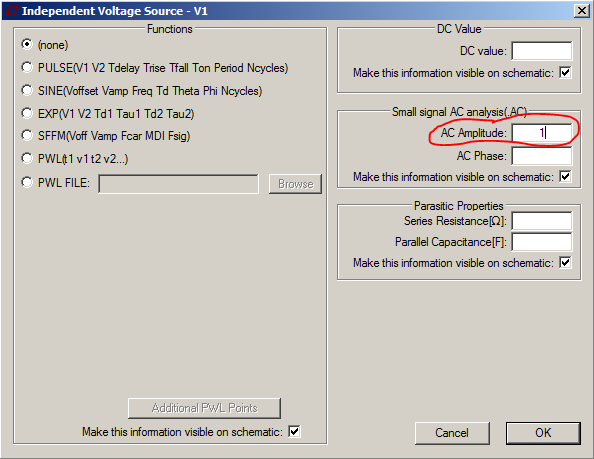
\includegraphics[width=0.7\textwidth]{figs/rc-ac0.PNG}
\caption{Резултати симулације \textit{RC} кола}
\label{Fig:rc-ac0}
\end{figure}

Сљедећи корак је дефинисати одговарајући тип симулације. Десним кликом на постојећи и избором језичка \texttt{AC Analysis}, добија се одговарајући дијалог. Унијети податке као на слици~\ref{Fig:rc-ac1}.

\begin{figure}[h]
\centering
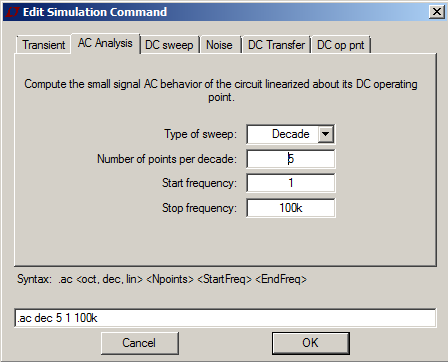
\includegraphics[width=0.7\textwidth]{figs/rc-ac1.PNG}
\caption{Резултати симулације \textit{RC} кола}
\label{Fig:rc-ac1}
\end{figure}

Коначан изглед шеме и графички приказ добијених резултата дат је на слици~\ref{Fig:rc-ac2}. Пуна линија представља магнитуду одзива (ордината лијево), док црткана линија представља фазну маргину одзива (ордината десно).

\begin{figure}[h]
\centering
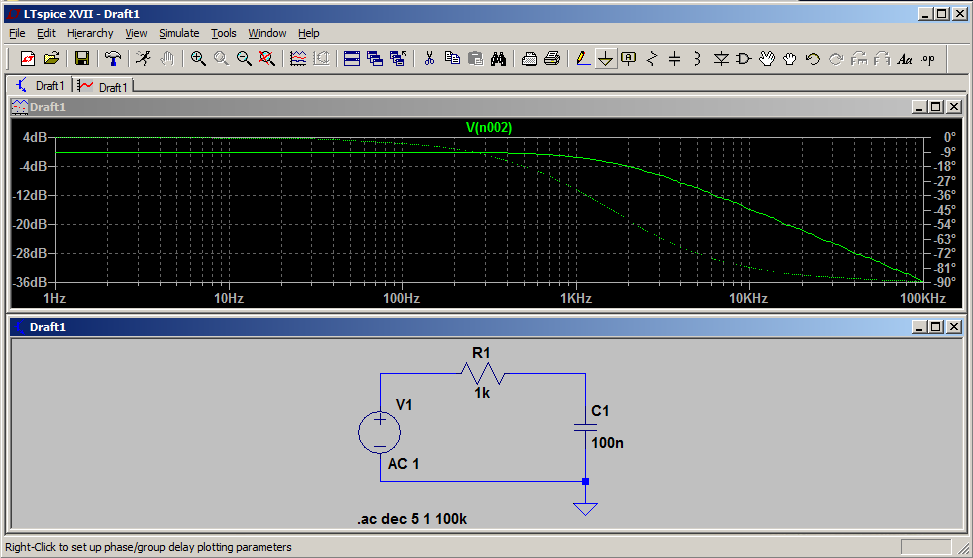
\includegraphics[width=\figwidth\textwidth]{figs/rc-ac2.PNG}
\caption{Резултати симулације \textit{RC} кола}
\label{Fig:rc-ac2}
\end{figure}

\chapter{Енкапсулација и тестно коло}

Елементе сваке од шема до сада посматраних могуће је, према намјени сваког елемента, подијелити на два скупа:
\begin{itemize}
\item елементи кола које обавља функцију (нпр. отпорници раздјелника напона са слике~\ref{Fig:rn-dc2}), и
\item елементи кола које задаје побуду и омогућава очитавање одзива (нпр. напонски извор са слике~\ref{Fig:rn-dc2}).
\end{itemize}

\section{Енкапсулација}

Један основних принципа објектно оријентисаног програмирања јесте енкапсулација. Ради се о јасном разграничењу између нивоа апстракције, чиме се постиже ефикаснији рад на сваком од њих. Преведено у контекст софтвера за цртање шема и симулатора, то значи да треба раздвојити коло које обавља функцију (у случају слике~\ref{Fig:rn-dc2}, функција је ,,дијељење напона''), од кола које задаје побуду и омогућава очитавање одзива.

Енкапсулација се, суштински, врши тако што се коло које обавља функцију замијени симболом, тј. цртежом одговарајућег облика, броја улазни и броја излазних приступа. Затим се, у новој шеми, тај симбол црта, као што се црта и симбол неког од стандардних елемената (отпорника или кондензатора), те му се задаје побуда, напајање и све што је потребно за омогућавање исправног рада и очитавања одзива. Симбол, у ствари, представља показивач на енкапсулирано коло.

На примјеру \textit{RC} кола са слике~\ref{Fig:rc-t0} показани су кораци за креирање симбола на основу нацртаног кола.

Први корак је цртање \textit{RC} кола у форми приказаној на слици~\ref{Fig:rc-symbol0}.

\begin{figure}[h]
\centering
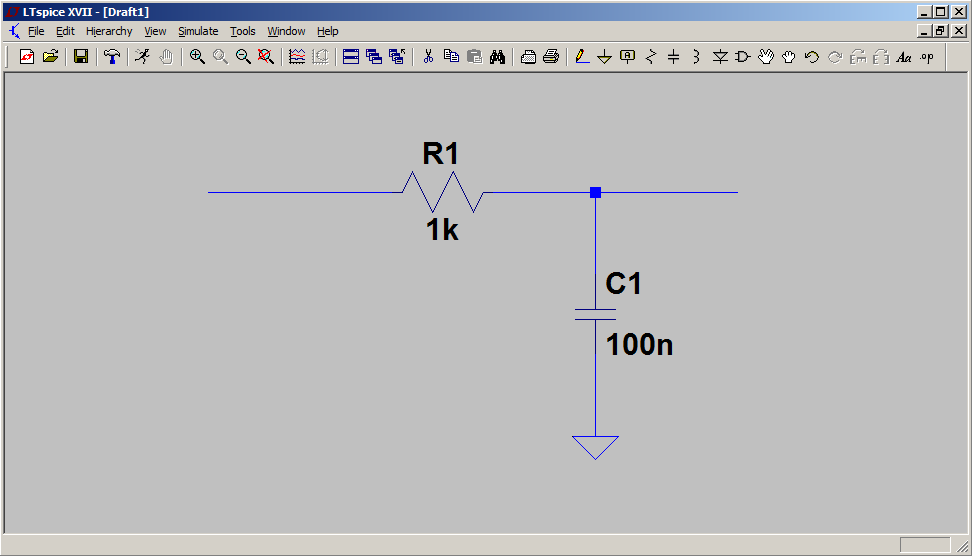
\includegraphics[width=\figwidth\textwidth]{figs/rc-symbol0.PNG}
\caption{Припрема за енкапсулацију - \textit{RC} коло}
\label{Fig:rc-symbol0}
\end{figure}

Потом је потребно назначити гдје се налазе улазни а гдје излазни приступи (енгл. \textit{pin} или \textit{port}, зависно од контекста). Притиском на \texttt{F4}, добија се прозор као на слици~\ref{Fig:rc-symbol1}, па се улазни приступ поставља подешавањима приказаним на слици~\ref{Fig:rc-symbol1}а, а излазни подешавањима приказаним на слици~\ref{Fig:rc-symbol1}б. Наравно, називи \texttt{ulaz} и \texttt{izlaz} су произвољни.

Након постављања опција као на слици~\ref{Fig:rc-symbol1}а, кликнути \texttt{OK} и креирани приступ поставити на одговарајуће мјесто. Исто поновити и након креирања излазног приступа, што би требало да резултује стањем приказаним на слици~\ref{Fig:rc-symbol2}.

\begin{figure}[h]
\centering
\begin{subfigure}{0.49\textwidth}
\centering
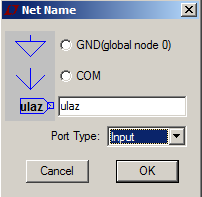
\includegraphics[width=0.8\textwidth]{figs/rc-symbol1a.PNG}
\caption*{а)}
\end{subfigure}
\begin{subfigure}{0.49\textwidth}
\centering
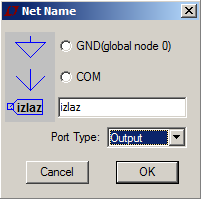
\includegraphics[width=0.8\textwidth]{figs/rc-symbol1b.PNG}
\caption*{б)}
\end{subfigure}
\caption{Постављање а) улазних и б) излазних приступа}
\label{Fig:rc-symbol1}
\end{figure}

\begin{figure}[h]
\centering
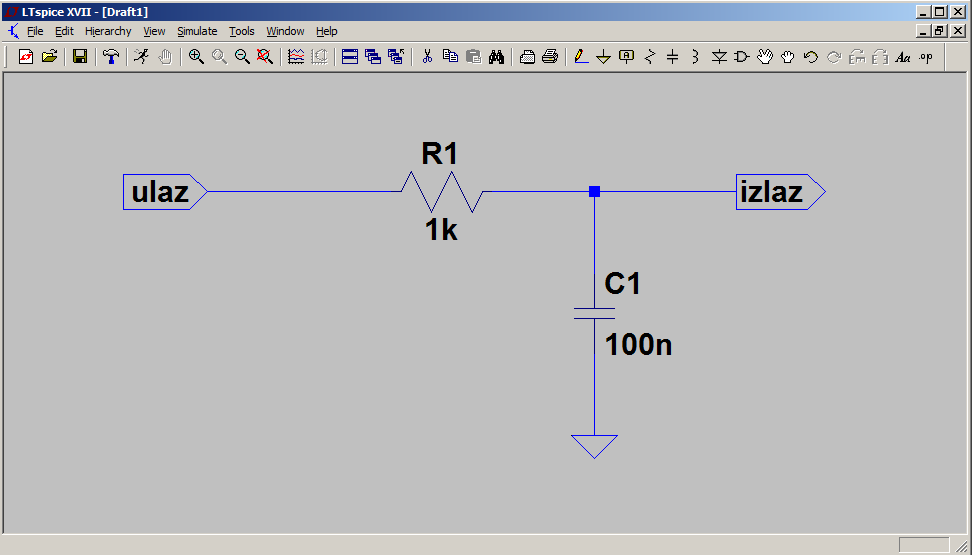
\includegraphics[width=\figwidth\textwidth]{figs/rc-symbol2.PNG}
\caption{Коначан изглед шеме \textit{RC} кола спремног за енкапсулацију}
\label{Fig:rc-symbol2}
\end{figure}

У складу са сликом~\ref{Fig:rc-symbol3}, из падајућег меније \textit{Hierarchy} изабрати опцију \textit{Open this Sheet's symbol}, па потврдно одговорити на питање које ће услиједити. Овим се креира симбол, а резултат је приказан на слици~\ref{Fig:rc-symbol5}.

\begin{figure}[h]
\centering
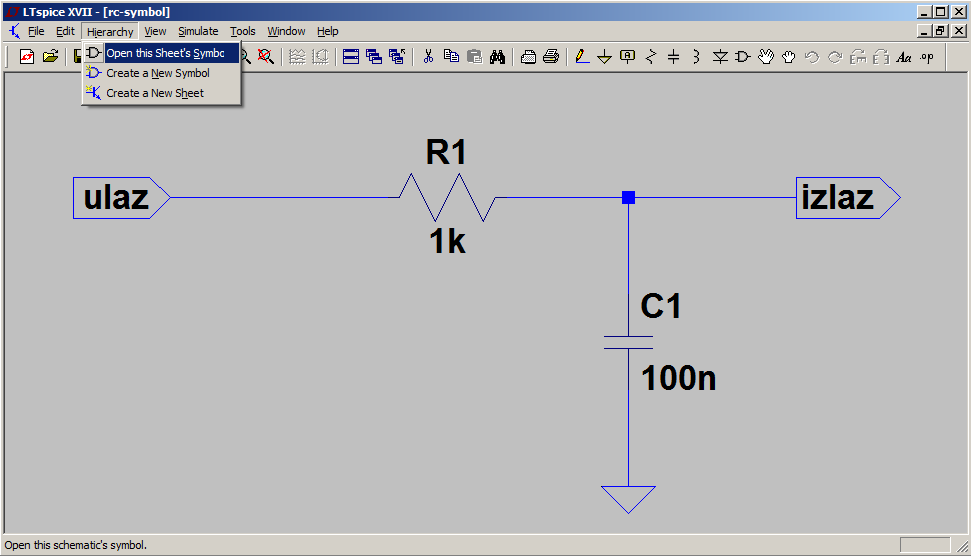
\includegraphics[width=\figwidth\textwidth]{figs/rc-symbol3.PNG}
\caption{Наредба за креирање симбола}
\label{Fig:rc-symbol3}
\end{figure}

\begin{figure}[h]
\centering
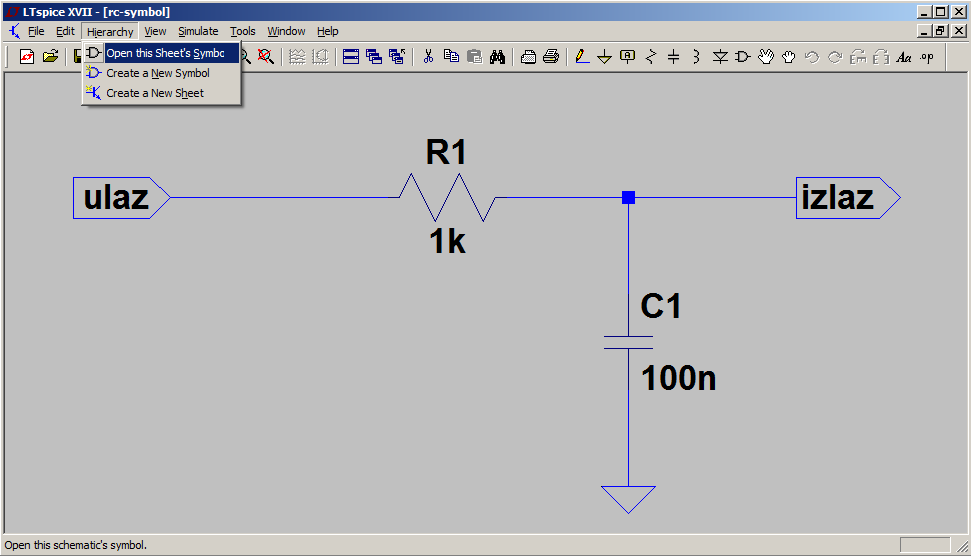
\includegraphics[width=\figwidth\textwidth]{figs/rc-symbol3.PNG}
\caption{Подразумијевани изглед симбола}
\label{Fig:rc-symbol5}
\end{figure}

Изглед симбола дат на слици~\ref{Fig:rc-symbol5} је подразумијеван и може се мијењати по потреби - у складу са намјеном кола које представља. У овом случају, нека симбол остане у подразумијеваној форми, само је неопходно сачувати га.

\section{Тестно коло}



\begin{figure}[h]
\centering
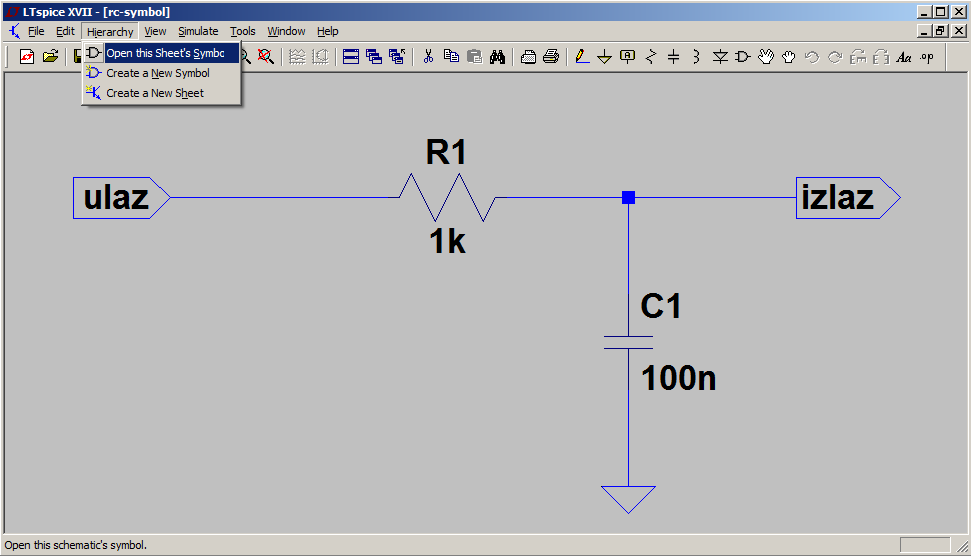
\includegraphics[width=\figwidth\textwidth]{figs/rc-symbol3.PNG}
\caption{Поставка за снимање струјно-напонске зависности диоде}
\label{Fig:rc-symbol6}
\end{figure}

\chapter{Примјене}

У овом одјељку, алати и вјештине научени у претходним примијењени су за рјешавање конкретних проблема.

\section{Снимање струјно-напонске зависности диоде}

Симбол диоде се додаје у шему притиском на тастер \texttt{D}, односно кликом на одговарајућу иконицу палете у врху прозора, десно. Користећи један од ова два начина и претходно стечена знања, нацртати шему као на слици~\ref{Fig:d-dc1}

\begin{figure}[h]
\centering
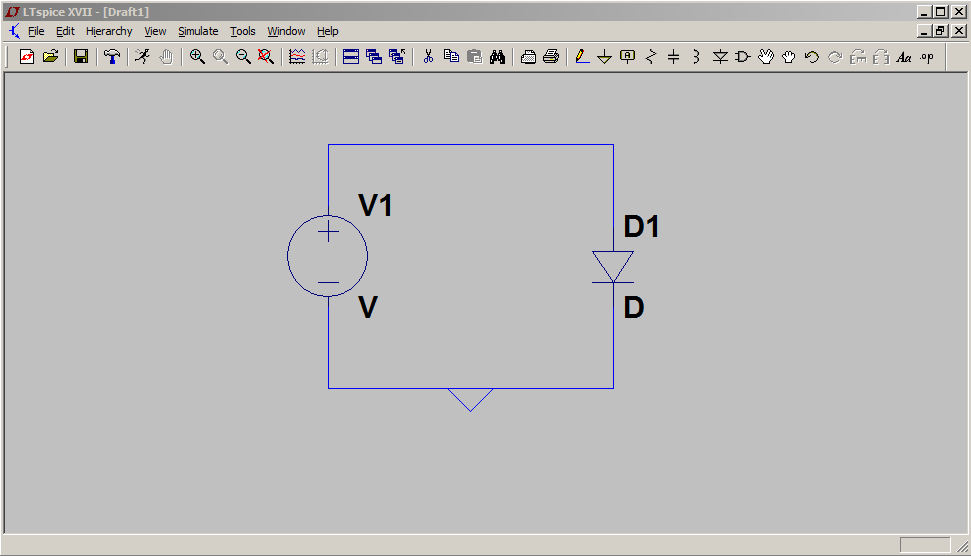
\includegraphics[width=\figwidth\textwidth]{figs/d-dc1.PNG}
\caption{Поставка за снимање струјно-напонске зависности диоде}
\label{Fig:d-dc1}
\end{figure}

Диода је нелинеаран елемнт, па је неопходно изабрати модел који описује његово понашање. Кликом десног тастера миша на симбол диоде добија се дијалог са слике~\ref{Fig:d-dc2}. Кликом на \textit{Pick New Diode} се добија на увид библиотека тренутно доступних модела, као што је приказано на слици~\ref{Fig:d-dc3}.

\begin{figure}[h]
\centering
\includegraphics[width=0.5\textwidth]{figs/d-dc2.PNG}
\caption{Својства симбола диоде}
\label{Fig:d-dc2}
\end{figure}

\begin{figure}[h]
\centering
\includegraphics[width=\figwidth\textwidth]{figs/d-dc3.PNG}
\caption{Списак доступних модела диоде}
\label{Fig:d-dc3}
\end{figure}

Изабрати ознаке \texttt{1N4148} и кликнути \texttt{OK}. Избор је могућ и двоструким кликом на ставку у табели. Сада шема изгледа као на слици~\ref{Fig:d-dc4}

\begin{figure}[h]
\centering
\includegraphics[width=\figwidth\textwidth]{figs/d-dc4.PNG}
\caption{Поставка за снимање струјно-напонске зависности диоде - модел диоде дефинисан}
\label{Fig:d-dc4}
\end{figure}

Симбол компоненте је, дакле, само показивач на структуру података која ће симулатору пренијети информацију о понашању електронске компоненте. Таква структура података назива се модел.

На слици~\ref{Fig:d-dc5} приказан је коначан изглед шеме - након што је дефинисан генератор и тип симулације - али и струјно-напонска карактеристика.

\begin{figure}[h]
\centering
\includegraphics[width=\figwidth\textwidth]{figs/d-dc5.PNG}
\caption{Струјно-напонска зависност диоде}
\label{Fig:d-dc5}
\end{figure}

На основу слике~\ref{Fig:d-dc5} и знања стечених у одјељку~\ref{dc}, дефинисати генератор и тип симулације тако да се добије исти, или довољно сличан, резултат.

\section{Одзив полуталасног исправљача на простопериодичну побуду}
\label{hwr}

Шема полуталасног исправљача дата је на слици~\ref{Fig:hwr-tran0}.

\begin{figure}[h]
\centering
\includegraphics[width=\figwidth\textwidth]{figs/hwr-tran0.PNG}
\caption{Струјно-напонска зависност диоде}
\label{Fig:hwr-tran0}
\end{figure}

За реализацију простопериодичне побуде потребно је прилагодити напонски генератор на начин приказан на слици~\ref{Fig:hwr-tran1}. Кључни параметри су амплитуда и учестаност, а могуће је додати и друге, као што је једносмјерна компонента.

\begin{figure}[h]
\centering
\includegraphics[width=0.7\textwidth]{figs/hwr-tran1.PNG}
\caption{Струјно-напонска зависност диоде}
\label{Fig:hwr-tran1}
\end{figure}

Дефинисати тип симулације и додијелити називе чворовима као на слици~\ref{Fig:hwr-tran2}. Покретање симулације даје одзив полуталасног исправљача на простопериодичну побуду - на истој слици.

\begin{figure}[h]
\centering
\includegraphics[width=\figwidth\textwidth]{figs/hwr-tran2.PNG}
\caption{Струјно-напонска зависност диоде}
\label{Fig:hwr-tran2}
\end{figure}


%\printbibliography 

\section*{}
\includepdf{pdfs/shortcuts.pdf}
\end{document}
